

\documentclass[a4paper]{article}
\usepackage{tikz}
\usetikzlibrary{calc}
\usepackage{amsmath}


\begin{document}

\section{Approach vector}
\begin{figure}[h!]
 \begin{center}
  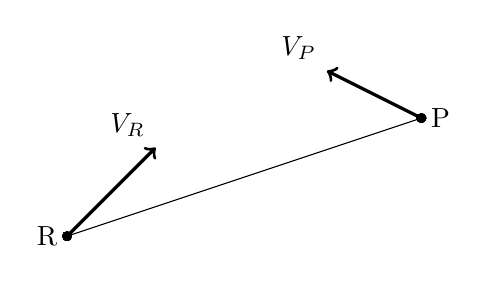
\begin{tikzpicture}[scale=1.5]
     \coordinate (RA) at (0.0, 0.0);
     \coordinate (RB) at (1.5, 1.5);
     \coordinate (PA) at (3.0, 1.0);
     \coordinate (PB) at (2.0, 1.5);

     \draw plot[mark size=1pt,mark=*] (RA) node[left] at (RA) {R};
     \draw plot[mark size=1pt,mark=*] (PA) node[right] at (PA) {P};
     \draw [black] (RA) -- (PA);
     \draw [->,black, very thick] (RA) -- ($(RA)!0.5!(RB)    $) node[above left] {$V_R$};
     \draw [->,black, very thick] (PA) -- ($(PA)!0.8!(PB)    $) node[above left] {$V_P$};

  \end{tikzpicture}
 \end{center}
\end{figure}

$$
   V_{rel} = \frac{(\overline{V}_R-\overline{V}_P)\cdot\overline{RP}}{|\overline{RP}|}
$$


\section{Closest approach}
\begin{figure}[h!]
 \begin{center}
  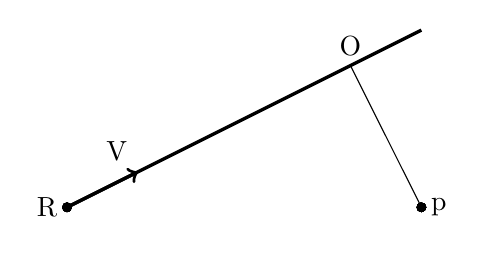
\begin{tikzpicture}[scale=1.5]
     %\draw[step=0.25cm,very thin,color=blue!20] (-0.5,-0.5) grid (3.5,2.0);
     \coordinate (A) at (0.0, 0.0);
     \coordinate (P) at (3.0, 0.0);
     \coordinate (C) at (3.0, 1.5);

     \draw plot[mark size=1pt,mark=*] (A) node[left] at (A) {R};
     \draw plot[mark size=1pt,mark=*] (P) node[right] at (P) {p};
     \draw [black, very thick] (C) -- (A);
     \draw [->,black, very thick] (A) -- ($(A)!0.2!(C)    $) node[above left] {V};
     \draw[black] (P) -- ($(A)!(P)!(C)$);
     \node[above] at ($(A)!(P)!(C)$) {O};

  \end{tikzpicture}
 \end{center}
\end{figure}


\newcommand\vOR{\overline{OR}}
\newcommand\vOP{\overline{OP}}
\newcommand\vP{\overline{P}}
\newcommand\vR{\overline{R}}
\newcommand\vV{\overline{V}}


$$
    l_j = \bar{x}_j + \bar{v}_j\cdot t    \qquad  p_i= \bar{x}_i
$$

$$
       \vOR\cdot \vOP = 0
$$

$$
   \overline{O}(t) = \binom{O_x}{O_y} = \binom{R_x + V_x\cdot t}{R_y+V_y\cdot t }, (t\ne 0)
$$

$$
       \vOR = \binom{R_x -(R_x + V_x\; t)}{R_y - (R_y+V_y\; t)} = \binom{-V_x\cdot t}{-V_y\cdot t} = - \overline{V} \; t
$$

$$
       \vOP = \binom{P_x -(R_x + V_x\; t)}{P_y-(R_y+V_y\; t)} = \overline{P}-\overline{R} - \overline{V}\; t
$$

\begin{eqnarray*}
    && \vOR\cdot \vOP=  0 \\
    &\Rightarrow& (\vP-\vR - \vV\; t) \cdot (- \vV \; t) = 0 \\
    &\Rightarrow& |V|^2t^2 - \vP\cdot \vV\; t + \vR\cdot \vV\; t = 0\\
     &\Rightarrow&  |V|^2t + (\vR-\vP)\cdot \vV\;  = 0  \\
  &\Rightarrow & t = \frac{(\vP-\vR)\cdot\vV}{|V|^2}
\end{eqnarray*}

\end{document}